\documentclass{beamer}
\usetheme{Berlin}
\usecolortheme{beaver}
\usepackage[ngerman]{babel}
\usepackage{graphicx}
\usepackage[utf8]{inputenc}
\usepackage{times}
\usepackage[T1]{fontenc}

\title{Malware}
\author{}
\date{}

\begin{document}

\maketitle
\begin{frame}
	\frametitle{Inhalt}
	\begin{enumerate}
		\item Viren und Würmer
		\item Trojaner
		\item Malware Protection
	\end{enumerate}
\end{frame}


\section{Viren und Würmer}
\begin{frame}
	\frametitle{Viren}
		\begin{block}{Geschichtliches:}
			\begin{itemize}
				\item 1949 Idee, dass ein Computerprogramm sich selbst wieder herstellen kann
				\item 1950 Idee in Spiel umgesetzt
				\item 1982 wurde erster Bootsektorvirus programmiert
				\item 1985-1990 wurden  MS-DOS, Apple Macintosh, Amiga, Atari und Unix opfer von ersten Virenangriffen
				$\Rightarrow$ Ersten Antivirenprogramme entwickelt
				\item 1990-1995 DOS-Viren
				\item 1995-2002 32-Bit-Windows Viren
				\item ab 2002 Anfang der Würmer
			\end{itemize}
		\end{block}
\end{frame}

\begin{frame}
	\frametitle{Viren}
		\begin{block}{Was sind Viren:}
			\begin{itemize}
				\item Verbreiten sich, indem es sich in noch nicht infizierte Dateien kopiert und diese dann ausgeführt werden.
				\item Diese Kopien haben folgenden Ziele:
				\begin{enumerate}
					\item Ausführen von Schadcode
					\item Weiteres Eindringen in andere Ressourcen des Computers
				\end{enumerate}
			\end{itemize}
		\end{block}
\end{frame}

\begin{frame}
	\frametitle{Viren}
		\begin{block}{Datei-Viren:}
			\begin{itemize}
				\item Am häufigsten anzutreffende Virentyp
				\item Virus muss sich in diese Wirtsdatei einfügen (oft am Ende)
				\item Wirtsdatei wird so modifiziert, dass das Virus beim Programmstart aufgerufen wird
				\item Eindringen auf unterschiedliche Art und Weise in ausführbaren Dateien
			\end{itemize}
		\end{block}
\end{frame}

\begin{frame}
	\frametitle{Viren}
		\begin{block}{Bootsektor-Viren:}
			\begin{itemize}
				\item Sind die ältesten Viren
				\item Bootsektoren von Disketten bzw. Festplatten werden infiziert
				\item Bootsektor wird bei jeden Start des Betriebssystems ausgeführt
				\item Heutzutage aber so gut wie Ausgestorben
			\end{itemize}
		\end{block}
\end{frame}

\begin{frame}
	\frametitle{Viren}
		\begin{block}{Marko-Viren:}
			\begin{itemize}
				\item Sind nicht eigenständige Programme, sondern in Form von Makros
				\item Makros sind Programme, die in Dokumenten eingebettet sind
				\item Darunter fallen: Microsoft Word, Microsoft Excel, Microsoft PowerPoint ...
				\item Meistens Ziel, die Standardvorlage zu infizieren da diese bei jedem Programmstart automatisch geladen wird und der Virus so automatisch mit aktiv wird
			\end{itemize}
		\end{block}
\end{frame}

\begin{frame}
	\frametitle{Viren}
	\begin{block}{Berühmte Viren:}
		\begin{itemize}
			\item Das Jerusalem-Virus
			\item Das Michelangelo-Virus
			\item Das Concept-Virus
		\end{itemize}
	\end{block}			
\end{frame}

\begin{frame}
	\frametitle{Würmer}
		\begin{block}{Geschichtliches:}
			\begin{itemize}
				\item 1997 verbreitet sich der erste E-Mail-Wurm Namens ShareFun
				\item 1999 verbreitet sich Über E-Mail der Wurm Melissa weltweit
				\item 2001 erscheinen erste Würmer mit einer eigenen SMTP-Engine
				\item 2005 erscheint mit SymbOS.Commwarrior der erste Wurm, der sich selbst als MMS verschicken kann
			\end{itemize}
		\end{block}
\end{frame}

\begin{frame}
	\frametitle{Würmer}
		\begin{block}{Was sind Würmer?}
			\begin{itemize}
				\item Im Gegensatz zu Viren dringen Würmer aktiv auf neue Systeme ein
				\item Nutzen Sicherheitslücken des Betriebssystems aus wie Netzwerkdienste oder Anwendungen die Netzwerkdienste beanspruchen
				\item Ein Wurm kann sich wie ein Virus in andere Programmdateien einnisten
			\end{itemize}
		\end{block}
\end{frame}

\begin{frame}
	\frametitle{Würmer}
		\begin{block}{E-Mail-Würmer:}
			\begin{itemize}
				\item Benutzen zur Verbreitung E-Mail Dienste
				\item Versenden E-Mail mit einer Datei oder einem Link als Anhang
				\item Durchsucht E-Mail Kontaktliste und versendet sich selbständig weiter
			\end{itemize}
		\end{block}
\end{frame}

\begin{frame}
	\frametitle{Würmer}
		\begin{block}{IM- und IRC-Würmer:}
			\begin{itemize}
				\item Benutzen zur Verbreitung Whatsapp, ICQ, MSN Messenger oder IRC-Clients
				\item Ähnlich wie bei E-Mail-Würmer versendet dieser einen Link an andere Kontakte mit der Schadhaften Datei
				\item Durchsucht Kontaktliste und versendet sich selbständig weiter
			\end{itemize}
		\end{block}
\end{frame}

\begin{frame}
	\frametitle{Würmer}
		\begin{block}{Berühmte Würmer:}
			\begin{itemize}
				\item Melissa
				\item Der Sasser-Wurm
				\item ILOVEYOU
				\item irgendwos mit D
			\end{itemize}
		\end{block}
\end{frame}


\section{Trojaner}
\begin{frame}
	\frametitle{Trojaner}
	\begin{enumerate}
		\item Geschichte 
		\item Was sind Trojaner
		\item Verbreitung
		\item Was ist ihr Ziel
		\item Bundestrojaner 
	\end{enumerate}
\end{frame}

\begin{frame}
	\frametitle{Geschichte}
	\begin{itemize}
		\item Name stammt vom Sieg der Griechen im Kampf gegen Troja
		\item Hölzernes Pferd mit Griechen darin
		\item Krieg gewonnen, weil sie unbemerkt in Troja waren
	\end{itemize}
	\flushright
	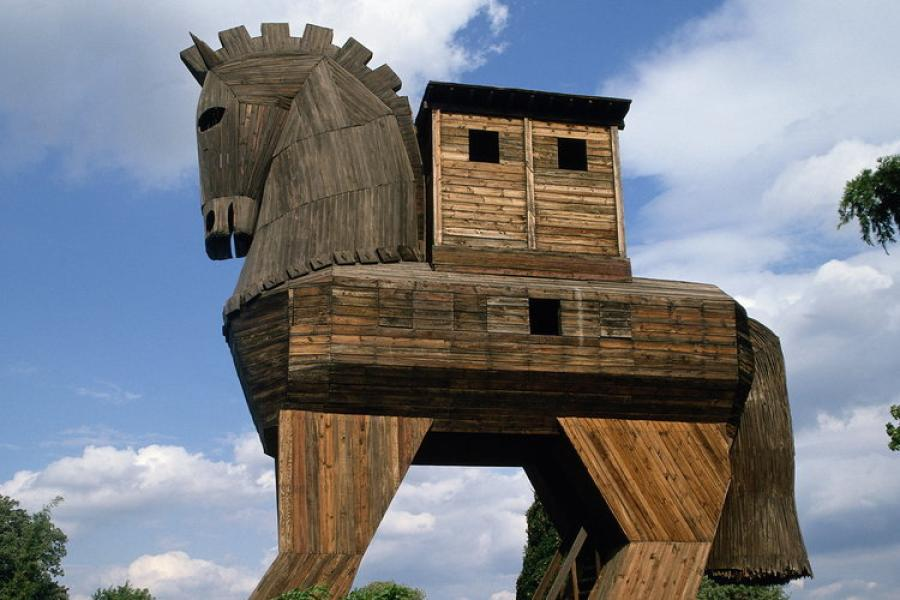
\includegraphics[width= 3.5cm]{bilder/pferd.jpg}
\end{frame}

\begin{frame}
	\frametitle{Was sind Trojaner?}
	\begin{itemize}
		\item Programme, die gezielt in Computer eingeschleust werden
		\item als nützliches Programm oder Software getarnt
		\item kann wirklich nützliche Funktionen enthalten
		\item Virus schon im Programm oder erst aus Internet heruntergeladen
		\item keine Weiterverbreitung im Gegensatz zu Viren und Würmern
	\end{itemize}
\end{frame}

\begin{frame}
	\frametitle{Was sind Trojaner?}
	\begin{itemize}
		\item keine selbstständige Reproduktion
		\item Schadprogramm läuft eigenständig auf PC
		\item Start der Schadsoftware
		\begin{enumerate}
			\item mit PC
			\item mit bestimmten Programm
		\end{enumerate}
		\item löschen und beenden funktioniert nicht 
	\end{itemize}
\end{frame}

\begin{frame}
	\frametitle{Verbreitung von Trojaner}
	\begin{itemize}
		\item mittels E-Mail (Anhang)
		\item P2P Websites und diverse Websites
		\item Werbe-CDs
		\item USB
	\end{itemize}
\end{frame}


\begin{frame}
	\frametitle{Aktivitäten der Schädlinge}
	Es werden meist unbemerkt Aktionen durchgeführt, wie zb Daten sammeln, welche im Internet übermittelt werden.
	\begin{itemize}
		\item Spionage
		\item Daten Diebstahl
		\item bis zu Zerstörung vom System
	\end{itemize}
\end{frame}

\begin{frame}
	\frametitle{Arten von Trojanern}
	\begin{itemize}
		\item Sniffer
		\begin{enumerate}
			\item aufzeichnen, auswerten, übertragen
			\item Keylogger
			\item Passwortspionage 
		\end{enumerate}
		\item Backdoor
		\begin{enumerate}
			\item Kontrolle wird übergeben
			\item Hacker kann alle Aktionen ausführen
			\item Zusammenschluss krimineller Zwecke
		\end{enumerate}
		\item Dropper
		\begin{enumerate}
			\item installiert andere Schadsoftware
			\item versteckt Schädlingsprogramme 
		\end{enumerate}
		\item Linker
		\begin{enumerate}
			\item verbindet schädliche Trojaner oder Programme
			\item nicht sichtbar auf PC
		\end{enumerate}
	\end{itemize}
\end{frame}

\begin{frame}
	\frametitle{Arten von Trojanern}
	\begin{itemize}
		\item Exploit
		\item Rootkit
		\item Trojan Banker
		\item Werbe- Trojaner
	\end{itemize}
	\flushright
	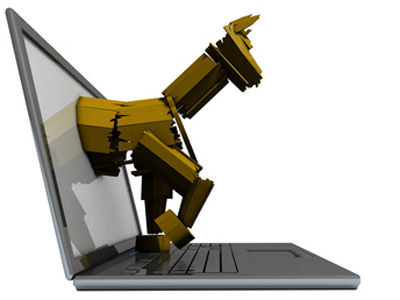
\includegraphics[width= 4cm]{bilder/trojaner.jpg}
\end{frame}

\begin{frame}
	\frametitle{Erkennung von Trojanern}
	Windows:
	\begin{itemize}
		\item beenden, herunterfahren
		\item Taskleiste verbirgt sich
		\item seltsame Meldungen in Dialogfenster
		\item Systemfarben ändern sich
		\item Laufwerke öffnen und schließen sich
	\end{itemize}
	OSX und Linux:
	\begin{itemize}
		\item Malware ist nicht so stark verbreitet
	\end{itemize}
\end{frame}


\begin{frame}
	\frametitle{Bundestrojaner}
	\begin{itemize}
		\item Online Durchsuchung
		\item staatliche Spähsoftware zur Strafverfolgung
		\item Kommunikationsnetzwerke werden durchsucht vom Staat
		\item kann mehr als nur Telekommunikation aufzuzeichnen
		\item gesamte Daten auf Gerät erlangen oder manipulieren
	\end{itemize}
\end{frame}

\begin{frame}
	\frametitle{Bundestrojaner Deutschland}
	\begin{enumerate}
		\item Rechtsgrundlage nochmals verändert nach Terroranschlägen
		\item 2009 - Wohnungen überwacht
		\item Telefonate belauscht
		\item Reformiertes BKA Gesetz - Grundlage für Bundestrojaner
		\item jahrelanger Rechtsstreit - Bestandteile BKA verfassungswidrig 
		\item Schutz von Privatsphäre nicht gesichert
		\item Beweise von Spionage können vor Gericht verwendet werden
		\item nur Daten aus laufenden Telekommunikationen 
	\end{enumerate}
\end{frame}


\begin{frame}
	\frametitle{Bundestrojaner Österreich}
	\begin{enumerate}
	\item 2007 Schadsoftware von DigiTask erworben
	\item diskusion über Zulassung in Österreich
	\item gegen Terror und Mordvergehen
	\item Whatsapp und Skype 
	\item noch keine gesetzes Grundlage 
	\item Einsatz der Software nicht geplant
	\end{enumerate}
	\flushright
	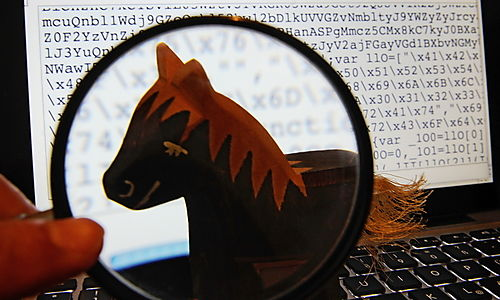
\includegraphics[width= 3.5cm]{bilder/oesterreich.jpg}
\end{frame}


\section{Malware Scanning}
\begin{frame}
\frametitle{Malware Scanning}

\begin{block}{Themen:}
\begin{enumerate}
\item Malware Statistik
\item Erkennungsrate vs. Infektionswahrscheinlichkeit
\item Performance-Efficiency-Tradeoff
\item Malware Scanning
\begin{itemize}
\item Static Scanning
\item Dynamic Scanning
\item Heuristic/Proactive Scanning
\end{itemize}
\end{enumerate}
\end{block}
\end{frame}

\begin{frame}
\frametitle{Statistik}

Neue Malware \\
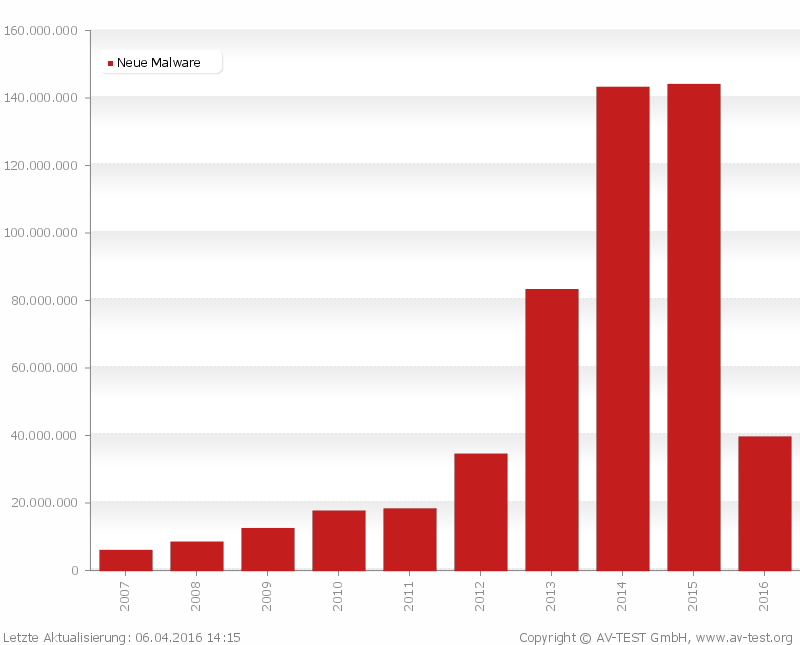
\includegraphics[height=6cm]{bilder/growth.png}
\end{frame}

\begin{frame}
\frametitle{Statistik}
Gesamte Malware \\
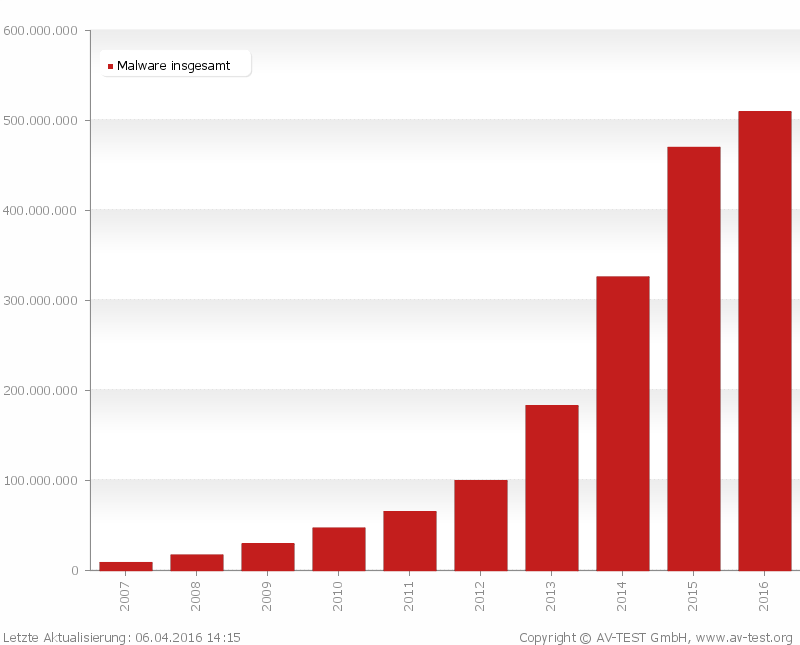
\includegraphics[height=6cm]{bilder/total.png}
\end{frame}

\begin{frame}
	\frametitle{Ransomware}
	\begin{block}{Definition}
		Wichtige persönliche Daten auf dem Computer der Opfers werden verschlüsselt und sind daher nicht mehr verwendbar.\\
		Den Entschlüsselungs-Key erhält man erst nach der Überweisung eines Lösegelds (ransom).
	\end{block}
\end{frame}
	

\begin{frame}
\frametitle{Statistik}
Ransomware \\
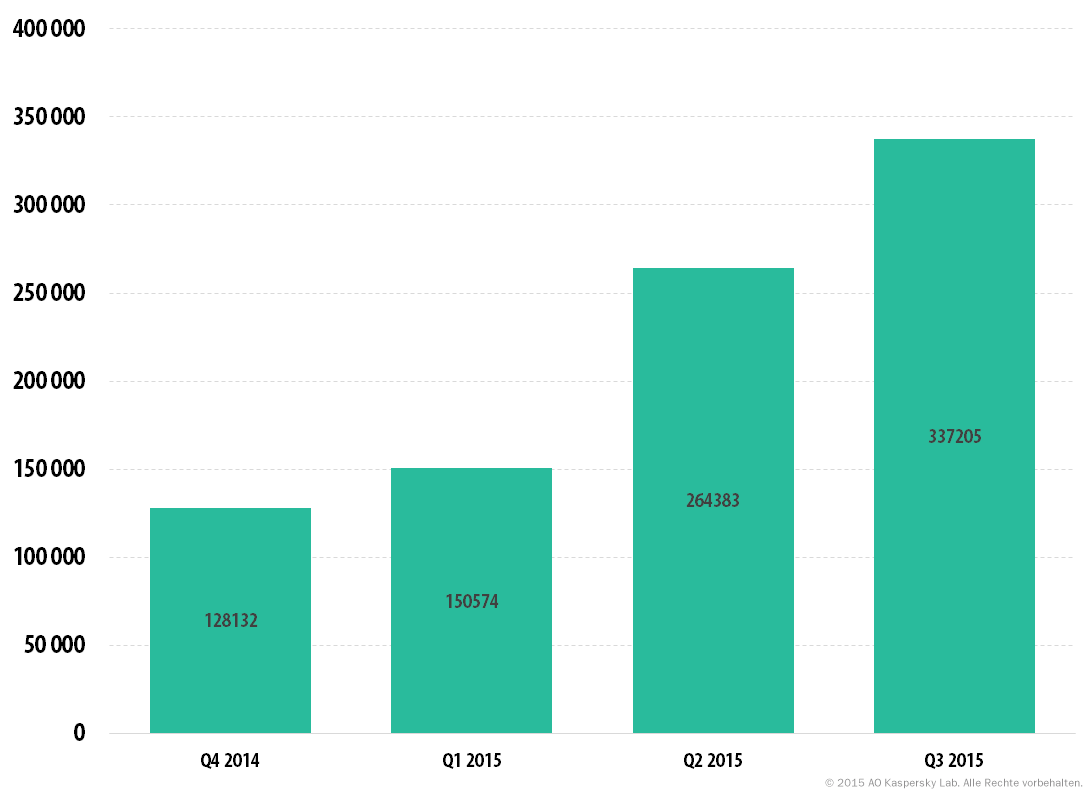
\includegraphics[height=6cm]{bilder/ransom.png}

\end{frame}


\begin{frame}
Hauptkriterien:
\begin{itemize}
	\item Erkennungsrate vs. Infektionswahrscheinlichkeit
	\item Performance-Effectivity-Tradeoff
	\item Scanning Techniken
\end{itemize}
\end{frame}

\begin{frame}
\frametitle{Erkennungsrate vs. Infektionswahrscheinlichkeit}
\begin{block}{}
	Infektionswahrscheinlichkeit != 1 - Erkennungsrate
\end{block}
Infektionswahrschinlichkeit bei $n$ voneinander unabhängigen Angriffen: \\
\centering
$p_{Befall} = (r_x)^n$
\end{frame}

\begin{frame}
\frametitle{Performance-Effectivity-Tradeoff}
Hohe Effektivität -> hoher Leistungsverbrauch -> niedrige Performance\\
Hohe Performance -> niedriger Leistungsverbrauch -> niedrige Effektivität

\begin{block}{}
	Kompromiss zwischen Performance und Effektivität
\end{block}
\end{frame}


\begin{frame}
\frametitle{Static Scanning}
\begin{block}{Static Scanning}
	\begin{enumerate}
		\item Codeausschnitt aus Datei
		\item Vergleich mit Codeausschnitten in Datenbank
		\item Entscheidung, ob Virus oder nicht
	\end{enumerate}
\end{block} 
\end{frame}

\begin{frame}
	\frametitle{Static Scanning}
	\begin{block}{Vorteile}
		\begin{itemize}
			\item Erkennt Malware mit festgelegter Signatur garantiert
			\item Datei muss nicht geöffnet/ausgeführt werden
		\end{itemize}
	\end{block} 
	\begin{block}{Nachteile}
		\begin{itemize}
			\item Übersieht unbekannte Schädlinge
			\item Erkennt keine alternativen Versionen
			\item Erkennt nur exakte Treffer
			\item Speicherverbrauch für Datenbank
		\end{itemize}
	\end{block}
\end{frame}

\begin{frame}
\frametitle{Dynamic Scanning}
\begin{block}{Dynamic Scanning}
	\begin{enumerate}
		\item Verhalten in Verhaltenskatalog gespeichert
		\item Überprüft Verhalten bei Öffnen/Ausführen
		\item Vergleicht Verhalten mit Katalog
		\item Blockiert Programm oder lässt Ausführung zu
	\end{enumerate}
	
\end{block} 
\end{frame}

\begin{frame}
	\frametitle{Dynamic Scanning}
	\begin{block}{Vorteile}
		\begin{itemize}
			\item Unbekannte Malware kann erkannt werden
		\end{itemize}
	\end{block} 
	\begin{block}{Nachteile}
		\begin{itemize}
			\item Schwierig alle Verhaltensweisen festzuhalten
			\item Kann evtl. Verhalten nicht erkennen
			\item Kann keine völlig neuen Schädlinge erkennen
			\item False-Positives: Blockiert gutartige Programme
		\end{itemize}
	\end{block}
\end{frame}


\begin{frame}
\frametitle{Heuristic/Proaktive Scanning}
\begin{block}{Heuristic/Proaktive Scanning}
	\begin{itemize}
		\item Bestimmt Wahrscheinlichkeit schädlichen Verhaltens
		\item Führt Datei nicht aus
		\item Blockiert Programm aufgrund berechneter Wahrscheinlichkeit
		\item Meist über Sandbox realisiert
	\end{itemize}
\end{block} 
\end{frame}

\begin{frame}
	\frametitle{Scanner umgehen}
	Malware kann nur gefunden werden wenn:
	\begin{itemize}
		\item Signatur in der Datenbank existiert
		\item Verhalten in der Datenbank existiert
		\item Heuristische Untersuchung eine hohe Wahrscheinlichkeit für schädliches Verhalten ermitteln
	\end{itemize}
	\pause
	Design neuer Malware:
	\begin{itemize}
		\item Neue Signatur oder komplett neues Verhalten kann von keinem Scanner erkannt werden
		\item Gefahr besteht, bis Änderungen in Anti-Malware integriert
		\item Integration von Signaturen schnell, von Verhaltensregeln langsam
		\item Bis zur Aktualisierung: kein Schutz
	\end{itemize}
\end{frame}



\begin{frame}
	\frametitle{Schlussfolgerung}
	Ein guter Scanner muss:
	\begin{itemize}
		\item alle Scanning-Techniken Kombinieren
		\item dadurch eine sehr hohe Erkennungsrate haben
		\item einen Kompromiss zwischen Performance und Effektivität finden
		\item Regelmäßig mit Updates versorgt werden
	\end{itemize}
\end{frame}

\begin{frame}
	\frametitle{Schlussfolgerung}
	\begin{block}{}
		Trotz der Erfüllung dieser Voraussetzungen sitzen Malware Entwickler immer am längeren Ast. Wird eine komplett neuartige Malware entwickelt, muss diese erst identifiziert, sowie Regeln und Signaturen dafür erstellt werden. Bis zu dem Zeitpunkt, zu dem das Update an User ausgeliefert wird, sind deren Geräte der neuen Malware schutzlos ausgeliefert
	\end{block}
\end{frame}

\end{document}
